\section{}
\[
H(s)=\frac{100\,s}{s+1}\,.
\]
\subsection{Bode-Diagramm}
\begin{center}
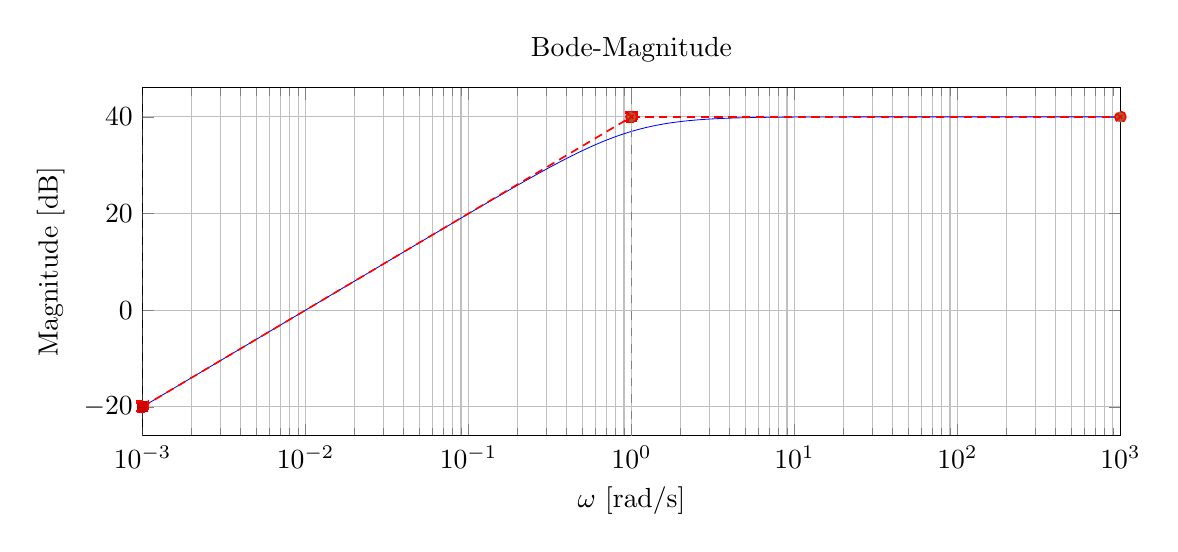
\begin{tikzpicture}
\begin{semilogxaxis}[
  width=14cm,height=6cm,
  xmin=1e-3,xmax=1e3,
  xlabel={$\omega$ [rad/s]},
  ylabel={Magnitude [dB]},
  grid=both,
  title={Bode-Magnitude}
]
\addplot[
  domain=1e-3:1e3,
  samples=600,
  mark=none,
  line width=0.3pt,
  blue
] {40 + 20*ln(x)/ln(10) - 20*ln(sqrt(1 + x^2))/ln(10)};
\addplot+[domain=1e-3:1,samples=2,dashed,dash pattern=on 3pt off 2pt,line width=0.6pt,red] {40 + 20*ln(x)/ln(10)};
\addplot+[domain=1:1e3,samples=2,dashed,dash pattern=on 3pt off 2pt,line width=0.6pt,red] {40};
\draw[gray,dashed] (rel axis cs:0,0) -- (rel axis cs:0,1);
\draw[gray,dashed] (axis cs:1,\pgfkeysvalueof{/pgfplots/ymin}) -- (axis cs:1,\pgfkeysvalueof{/pgfplots/ymax});
\node[gray,anchor=south east] at (axis cs:1,\pgfkeysvalueof{/pgfplots/ymax}) {\scriptsize Pol $\omega_p=1$};
\end{semilogxaxis}
\end{tikzpicture}
\vspace{6mm}
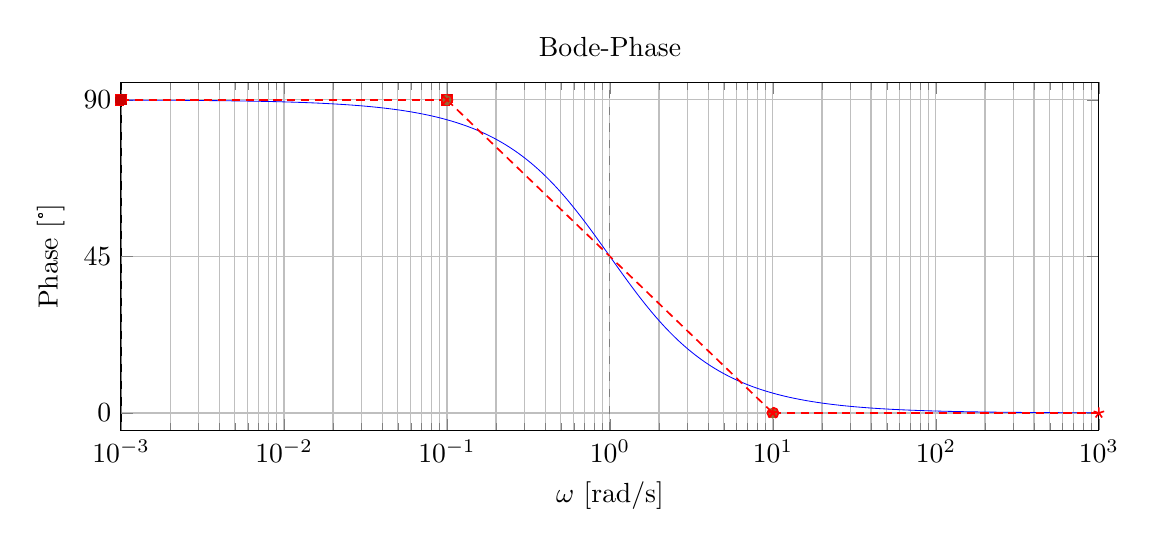
\begin{tikzpicture}
\begin{semilogxaxis}[
  width=14cm,height=6cm,
  xmin=1e-3,xmax=1e3,
  ymin=-5,ymax=95,
  xlabel={$\omega$ [rad/s]},
  ylabel={Phase [°]},
  grid=both,
  ytick distance=45,
  title={Bode-Phase}
]
\addplot[
  domain=1e-3:1e3,
  samples=600,
  mark=none,
  line width=0.3pt,
  blue
] {90 - atan(x)};
\addplot+[domain=1e-3:1e-1,samples=2,dashed,dash pattern=on 3pt off 2pt,line width=0.6pt,red] {90};
\addplot+[domain=1e-1:1e1,samples=2,dashed,dash pattern=on 3pt off 2pt,line width=0.6pt,red] {45 - 45*ln(x)/ln(10)};
\addplot+[domain=1e1:1e3,samples=2,dashed,dash pattern=on 3pt off 2pt,line width=0.6pt,red] {0};
\draw[gray,dashed] (rel axis cs:0,0) -- (rel axis cs:0,1);
\draw[gray,dashed] (axis cs:1,\pgfkeysvalueof{/pgfplots/ymin}) -- (axis cs:1,\pgfkeysvalueof{/pgfplots/ymax});
\node[gray,anchor=south east] at (axis cs:1,\pgfkeysvalueof{/pgfplots/ymax}) {\scriptsize Pol $\omega_p=1$};
\end{semilogxaxis}
\end{tikzpicture}
\end{center}
\newpage
\subsection{Erklärung (ausführlich)}
\begin{description}[leftmargin=1.2em,labelsep=.6em,font=\bfseries]

\item[1. Zuerst Normalform herstellen.]
\[
H(s)=\frac{100s}{s+1}=100\cdot s\cdot \frac{1}{\,(1+sT_p)}
\]
Die Teilglieder und Variablen gemäß Skript sind: 
\[
\underline{F}_1(s)=\frac{1}{1+s},\;T_p=1,\;K_0=100\;\text{und}\;r=0.
\]


\item[2. Danach Eckfrequenz bestimmen und sortieren.]
\[
\omega_p=\frac{1}{T_p}=1\,\mathrm{rad/s}.
\]
Diese ist die einzige Eckfrequenz, daher ist eine Sortierung der Eckfrequenzen hier hinfällig.

\item[3. Startpunkt des Amplitudengangs festlegen (Geradennäherung).]
Setze $\omega_{\min}=\omega_p=1$.
\[
F_{\mathrm{dB}}(\omega_{\min})=20\log_{10}\!\big(|K_0\,F^*_{ges}(0)|\,\omega_{\min}^{\,r}\big)
=20\log_{10}(100\cdot 1\cdot 1)=40\,\mathrm{dB}.
\]
Anfangssteigung $r\cdot 20\,\mathrm{dB/dec}=+20\,\mathrm{dB/dec}$.

\item[4. Verlauf links vom Startpunkt.]
Für $\omega<\omega_{\min}=1$ gilt die Geradennäherung mit Steigung $+20\,\mathrm{dB/dec}$. Einzeichnen als Gerade mit Steigung $+20\,\mathrm{dB/dec}$ durch den Punkt $(\omega_{\min},\,40\,\mathrm{dB})$.


\item[5. Steigungswechsel an der Eckfrequenz eintragen.]
$\underline{F}_2$ reduziert ab $\omega_p$ die Steigung um $20\,\mathrm{dB/dec}$:
\[
\omega<1:\ +20\,\mathrm{dB/dec},\qquad \omega\ge 1:\ 0\,\mathrm{dB/dec}.
\]

\item[6. Eckabrundung korrekt berücksichtigen.]
\[
|H(j\omega)|=\frac{100\,\omega}{\sqrt{1+\omega^2}},\qquad
|H(j\cdot 1)|_{\mathrm{dB}}=40-10\log_{10}2\approx 36.99\,\mathrm{dB}.
\]
Bei $\omega=1$ liegt die Kurve etwa $3.01\,\mathrm{dB}$ unter der rechten Asymptote.
\newpage
\item[7. Phasenstartwert festlegen.]
Da $K_0F_{\mathrm{ges}}(0)>0$ und $r=1$ gilt
\[
\varphi(0)=\arg\!\big(K_0F_{\mathrm{ges}}(0)\big)+r\cdot90^\circ
=0^\circ+1\cdot90^\circ=+90^\circ.
\]


\item[8. Phasenänderung durch die Teilglieder eintragen.]
für $\omega \ll 0.1$: konstante $+90^\circ$.
Wegen $\underline{F}_1$ (Pol 1. Ordnung) sinkt die Phase von $90^\circ\to 0^\circ$ über $[0.1,10]$ ab.
Geradennäherung gesamt:
\[
\varphi(\omega)\approx
\begin{cases}
+90^\circ,& \omega\le 0.1,\\
45^\circ-45^\circ\log_{10}\omega,& 0.1<\omega<10,\\
0^\circ,& \omega\ge 10.
\end{cases}
\]

\item[9. Grenzwerte und Konsistenz prüfen.]
DC: $|H(0)|=0\mathrel{\widehat{=}} -\infty\, \mathrm{dB},\ \varphi(0)=90^\circ$.
HF: $|H(j\omega)|\to 100\Rightarrow 40\,\mathrm{dB}$.

Pol-/Nullzählung: Zählergrad $m=1$, Nennergrad $n=1\Rightarrow \varphi(\infty)=(m-n)\cdot90^\circ=0^\circ$.
\end{description}

\subsubsection*{Stückweise Näherungen (für die Skizze)}
\[
|H(j\omega)|_{\mathrm{dB}}\approx
\begin{cases}
40+20\log_{10}\omega,& \omega\ll 1,\\[2pt]
40-10\log_{10}2,& \omega=1,\\[2pt]
40,& \omega\gg 1,
\end{cases}
\qquad
\varphi(\omega)\approx
\begin{cases}
+90^\circ,& \omega\le 0.1,\\[2pt]
45^\circ-45^\circ\log_{10}\omega,& 0.1<\omega<10,\\[2pt]
0^\circ,& \omega\ge 10.
\end{cases}
\]

\newpage